
\documentclass[a4paper,12pt]{article}
\usepackage[utf8]{inputenc}
\usepackage[T1]{fontenc}
\usepackage{graphicx}
\title{Esercizi Web Services - Pagine 63, 64, 65 e 68}
\author{}
\date{}

\begin{document}
\maketitle

\section*{Esercizio 1 (pagina 63)}
\begin{enumerate}
  \item Alla linea di comando vanno passati \texttt{tipofunzione op1 op2}.
  \item
    \begin{figure}[h]
      \centering
      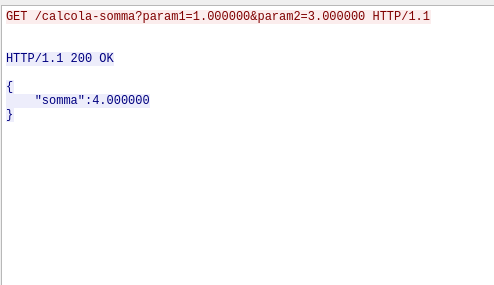
\includegraphics[width=0.6\linewidth]{wireshark.png}
      \caption{Scambio HTTP GET verso \texttt{/calcola-somma}}
    \end{figure}
    Si può notare che è una normale richiesta HTTP GET verso l’API \texttt{/calcola-somma}, mentre la risposta è in formato JSON.
  \item La signature di \texttt{calcoloSomma} è:
    \[
      \texttt{float calcoloSomma(float, float)}
    \]
    Averle uguali serve a mantenere lo stesso tipo e ordine dei parametri, evitando errori di interpretazione.
\end{enumerate}

\section*{Esercizio 2 (pagina 64)}
È un’opportunità, poiché:
\begin{itemize}
  \item Lo strato HTTP fa da “collante”, disaccoppiando completamente i binari: il contratto è solo sull’URL, sui parametri e sul payload.
  \item Libertà evolutiva: puoi riscrivere il server in Rust domani o aggiungere un client mobile in Kotlin senza toccare il resto.
\end{itemize}

\section*{Esercizio 3 (pagina 65)}
\begin{enumerate}
  \item
    \begin{figure}[h]
      \centering
      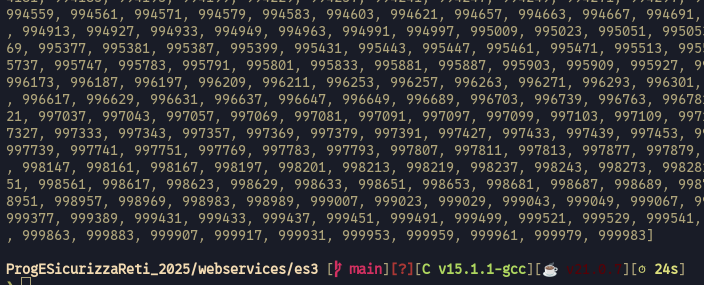
\includegraphics[width=0.6\linewidth]{timer.png}
      \caption{Tempo di calcolo dei numeri primi}
    \end{figure}
  \item No, non è stato necessario tradurre l’algoritmo dei numeri primi in Java, perché tutta la parte algoritmica e di calcolo è svolta interamente dal processo server. L'unica aggiunta in Java è la funzione che invia la richiesta.
\end{enumerate}

\section*{Esercizio Finale (pagina 68)}
\begin{enumerate}
  \item Basterebbe passare tre indirizzi diversi (che puntano a macchine con lo stesso servizio).
  \item No, purché ciascuna macchina esponga lo stesso servizio REST sulla porta 8000.
  \item Dividi lo spazio in N spezzoni uguali, ad esempio:
    \[
      \text{server A} \to [1..333333],\quad
      \text{server B} \to [333334..666666],\quad
      \text{server C} \to [666667..1000000].
    \]
  \item No, la parte logica del server fa già quello che deve fare: basta lanciare più istanze (su host o porte diverse).
\end{enumerate}

\end{document}
